%% ============================================================ 31  VJC 2025 Promo Q9(a),(b)
\defQ{31}{}{%
A curve $C$ has equation $y=\dfrac{x^{2}-4x+1}{x+1}$, $x\neq-1$.
\begin{qparts}
\pt{(a)} Prove, using an algebraic method, that $y=\dfrac{x^{2}-4x+1}{x+1}$ cannot lie between two certain values, to be determined in exact form. \mk{3}
\pt{(b)} Sketch $C$, stating the equations of any asymptotes, and the coordinates of any turning points and any axial intercepts. \mk{4}
\end{qparts}
\src{VJC 2025 Promo Q9(a), (b)}}
\defS{31}{%
\begin{gtpart}{(a)}{3}\begin{topalign}
y&=\frac{x^{2}-4x+1}{x+1}\\
yx+y&=x^{2}-4x+1\\
x^{2}+(-y-4)x+(1-y)&=0\\
\text{No real solution for }x:\quad(-y-4)^{2}-4(1-y)&<0\\
y^{2}+8y+16-4+4y&<0\\
y^{2}+12y+12&<0\\
(y+6)^{2}-24&<0\\
\left(y+6-\sqrt{24}\right)\left(y+6+\sqrt{24}\right)&<0\\
-6-2\sqrt6<y&<-6+2\sqrt6\\
\therefore\ y\text{ cannot lie between }&-6-2\sqrt6\ \text{and}\ -6+2\sqrt6
\end{topalign}\end{gtpart}
\begin{gtpart}{(b)}{4}\begin{topalign}
y&=x-5+\frac{6}{x+1}\\
\text{Asymptotes: }&x=-1,\ y=x-5\\
x=0:\ y&=1\\
y=0:\ x^{2}-4x+1=0\ \Rightarrow\ x&=0.268,\ 3.73\\
\text{Turning points: }&(1.45,-1.10),\ (-3.45,-10.9)
\end{topalign}
\begin{center}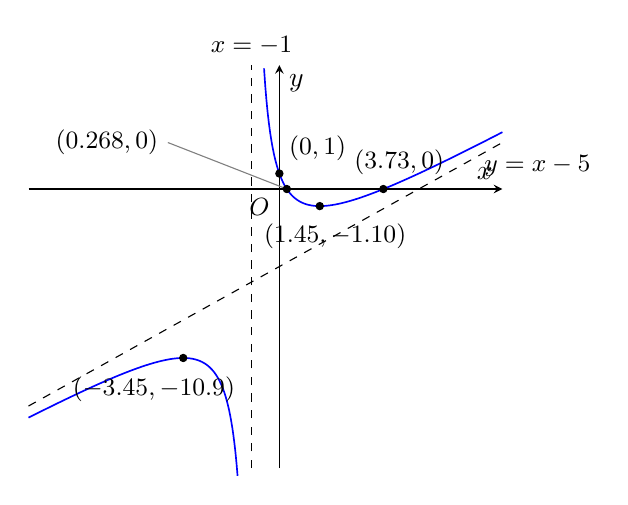
\begin{tikzpicture}
\begin{axis}[width=7.6cm,height=6.7cm,axis lines=middle,xmin=-9,xmax=8,ymin=-18,ymax=8,ticks=none,clip=false,xlabel=$x$,ylabel=$y$]
\addplot[black,dashed] coordinates{(-1,-18)(-1,8)};
\addplot[black,dashed,domain=-9:8]{x-5};
\addplot[blue,semithick,domain=-0.55:8,samples=200]{x-5+6/(x+1)};
\addplot[blue,semithick,domain=-9:-1.5,samples=200]{x-5+6/(x+1)};
\addplot[black,only marks,mark=*,mark size=1.3pt] coordinates{(0,1)(0.268,0)(3.73,0)(1.449,-1.101)(-3.449,-10.899)};
\node[font=\small,anchor=north east] at (axis cs:0,0){$O$};
\node[font=\small,anchor=south west] at (axis cs:0,1.2){$(0,1)$};
\node[font=\small,anchor=south] at (axis cs:4.3,0.3){$(3.73,0)$};
\draw[thin,gray] (axis cs:0.268,0)--(axis cs:-4,3);\node[font=\small,anchor=east] at (axis cs:-4,3){$(0.268,0)$};
\node[font=\small,anchor=north] at (axis cs:2,-1.6){$(1.45,-1.10)$};
\node[font=\small,anchor=north] at (axis cs:-4.5,-11.5){$(-3.45,-10.9)$};
\node[font=\small,anchor=south] at (axis cs:-1,8){$x=-1$};
\node[font=\small,anchor=west] at (axis cs:7,1.5){$y=x-5$};
\end{axis}\end{tikzpicture}\end{center}\end{gtpart}}
%% ============================================================ 32  SAJC 2025 Promo Q7
\defQ{32}{}{%
A curve $C$ has equation $y=ax+b+\dfrac{2b-a}{x+3}$, where $a$ and $b$ are constants such that $a>0$, $b\neq\dfrac12a$ and $x\neq-3$.
\begin{qparts}
\pt{(a)} If $C$ has no stationary points, use differentiation to find the relationship between $a$ and $b$. \mk{3}
\pt{(b)} It is now given that $b=a$.
\begin{qparts}
\pt{(i)} Find the $x$-coordinates of the turning points. \mk{2}
\pt{(ii)} Hence sketch $C$, stating the equations of any asymptotes and the coordinates of the axial intercepts and turning points. \mk{3}
\pt{(iii)} Verify that the point of intersection of the two asymptotes of $C$ lies on the line $y=kx+3k-2a$.\par
Hence, using the graph in part (b)(ii), find the range of values of $k$ in terms of $a$, such that the equation $x(k-a)+3k-2a-b-\dfrac{2b-a}{x+3}=0$ has real roots. \mk{2}
\end{qparts}
\end{qparts}
\src{SAJC 2025 Promo Q7}}
\defS{32}{%
\begin{qparts}
\pt{(a)} \begin{topalign}
\frac{\mathrm{d}y}{\mathrm{d}x}&=a-\frac{2b-a}{(x+3)^{2}}\\
\frac{\mathrm{d}y}{\mathrm{d}x}=0:\quad a-\frac{2b-a}{(x+3)^{2}}&=0\\
(x+3)^{2}&=\frac{2b-a}{a} &&---(1)\\
\text{No stationary points}\ \Rightarrow\ \frac{2b-a}{a}&<0\\
\text{Since }a>0,\quad 2b-a&<0\\
\therefore\ a&>2b
\end{topalign}
\pt{(b)(i)} \begin{topalign}
b=a:\quad (x+3)^{2}&=\frac{2a-a}{a}=1\\
x+3&=1\ \text{or}\ -1\\
x&=-2\ \text{or}\ -4
\end{topalign}
\pt{(b)(ii)} \begin{topalign}
y&=ax+a+\frac{a}{x+3}\\
\text{Asymptotes: }&x=-3,\ y=ax+a\\
x=-2:\ y=0;\quad x=-4:\ y&=-4a\\
\text{Turning points: }&(-2,0),\ (-4,-4a)\\
x=0:\ y&=\frac43a\\
y=0:\ ax+a+\frac{a}{x+3}=0\ \Rightarrow\ (x+1)(x+3)+1&=0\\
x^{2}+4x+4=0\ \Rightarrow\ (x+2)^{2}=0\ \Rightarrow\ x&=-2
\end{topalign}
\begin{center}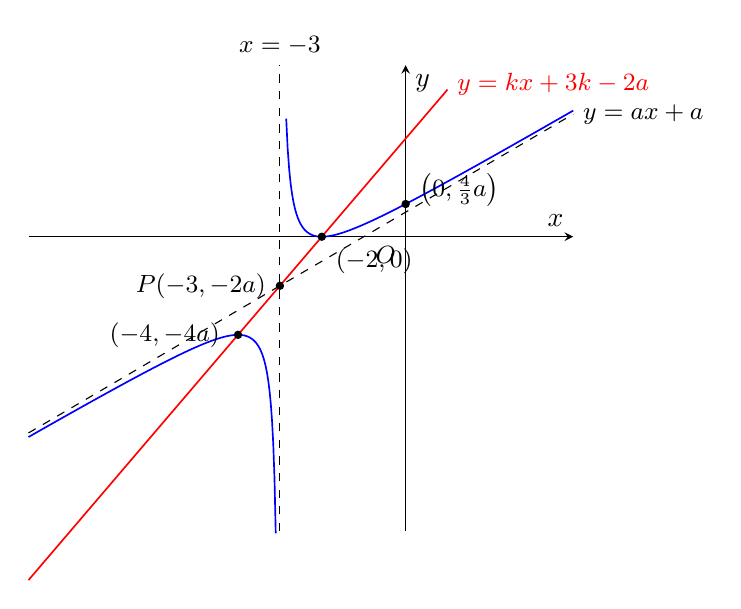
\begin{tikzpicture}
\begin{axis}[width=8.5cm,height=7.5cm,axis lines=middle,xmin=-9,xmax=4,ymin=-12,ymax=7,ticks=none,clip=false,xlabel=$x$,ylabel=$y$]
\addplot[black,dashed] coordinates{(-3,-12)(-3,7)};
\addplot[black,dashed,domain=-9:4]{x+1};
\addplot[blue,semithick,domain=-2.85:4,samples=200]{x+1+1/(x+3)};
\addplot[blue,semithick,domain=-9:-3.1,samples=200]{x+1+1/(x+3)};
\addplot[red,semithick,domain=-9:1]{2*(x+3)-2};
\addplot[black,only marks,mark=*,mark size=1.3pt] coordinates{(-2,0)(-4,-4)(0,1.333)(-3,-2)};
\node[font=\small,anchor=north east] at (axis cs:0,0){$O$};
\node[font=\small,anchor=north west] at (axis cs:-1.9,-0.1){$(-2,0)$};
\node[font=\small,anchor=east] at (axis cs:-4.2,-4){$(-4,-4a)$};
\node[font=\small,anchor=west] at (axis cs:0.1,1.9){$\left(0,\frac43a\right)$};
\node[font=\small,anchor=east] at (axis cs:-3.1,-2){$P(-3,-2a)$};
\node[font=\small,anchor=south] at (axis cs:-3,7){$x=-3$};
\node[font=\small,anchor=west] at (axis cs:4,5){$y=ax+a$};
\node[font=\small,anchor=west,red] at (axis cs:1,6.2){$y=kx+3k-2a$};
\end{axis}\end{tikzpicture}\end{center}
\pt{(b)(iii)} \begin{topalign}
x=-3\ \text{and}\ y=ax+a:\quad y&=-3a+a=-2a\\
\text{Intersection of asymptotes: }&P(-3,-2a)\\
x=-3:\quad \text{RHS}=k(-3)+3k-2a&=-2a=\text{LHS}\\
\therefore\ P\text{ lies on the line }&y=kx+3k-2a\\
x(k-a)+3k-2a-b-\frac{2b-a}{x+3}&=0\\
kx+3k-2a&=ax+b+\frac{2b-a}{x+3}\\
\text{Line through }P\text{ meets }C\ &\Rightarrow\ k>a
\end{topalign}
\end{qparts}}
%% ============================================================ 33  DHS 2025 Promo Q8
\defQ{33}{}{%
A curve $C$ has equation $\mathrm{f}(x)=\dfrac{3x^{2}+6x+k}{x+2}$, where $x>-2$ and $k$ is a non-zero real constant.\par
It is given that the function f is strictly increasing.
\begin{qparts}
\pt{(a)} Find the range of values of $k$. \mk{3}
\pt{(b)} Sketch the curve $C$, giving the coordinates of any points where $C$ crosses the $x$- and $y$-axes and the equations of any asymptotes. \mk{3}
\pt{(c)} By adding a suitable curve to the graph of the curve $C$ in (b), deduce the number of distinct real root(s) of the equation $\left(3x^{2}+6x+k\right)^{2}=\left(x^{2}+1\right)\left(9x^{2}+36x+36\right)$. \mk{3}
\end{qparts}
\src{DHS 2025 Promo Q8}}
\defS{33}{%
\begin{qparts}
\pt{(a)} \begin{topalign}
\mathrm{f}(x)&=\frac{3x^{2}+6x+k}{x+2}=3x+\frac{k}{x+2}\\
\mathrm{f}'(x)&=3-\frac{k}{(x+2)^{2}}=\frac{3x^{2}+12x+12-k}{(x+2)^{2}}\\
\text{f strictly increasing}\ \Rightarrow\ \mathrm{f}'(x)&>0\\
3x^{2}+12x+12-k&>0\quad\because\ (x+2)^{2}>0\ \text{for}\ x>-2\\
3(x+2)^{2}-k&>0\\
\text{Since }3(x+2)^{2}-k>-k\ \text{for all}\ x>-2,\quad -k&\geqslant0\\
k\neq0\ \Rightarrow\ k&<0
\end{topalign}
\pt{(b)} \begin{topalign}
y&=3x+\frac{k}{x+2}\\
\text{Asymptotes: }&y=3x,\ x=-2\\
x=0:\ y&=\frac{k}{2}\\
y=0:\ 3x^{2}+6x+k=0\ \Rightarrow\ x&=\frac{-6\pm\sqrt{36-12k}}{6}=-1\pm\frac{\sqrt{9-3k}}{3}\\
x>-2\ \Rightarrow\ x&=-1+\frac{\sqrt{9-3k}}{3}
\end{topalign}
\pt{(c)} \begin{topalign}
\left(3x^{2}+6x+k\right)^{2}&=\left(x^{2}+1\right)\left(9x^{2}+36x+36\right) &&---(*)\\
\left(3x^{2}+6x+k\right)^{2}&=9\left(x^{2}+1\right)(x+2)^{2}\\
\left(\frac{3x^{2}+6x+k}{x+2}\right)^{2}-9x^{2}&=9\\
\text{Draw the hyperbola }\ \frac{y^{2}}{3^{2}}-\frac{x^{2}}{1^{2}}&=1\\
\text{Asymptotes }y=\pm3x,\ \text{vertices }&(0,\pm3)
\end{topalign}
\begin{center}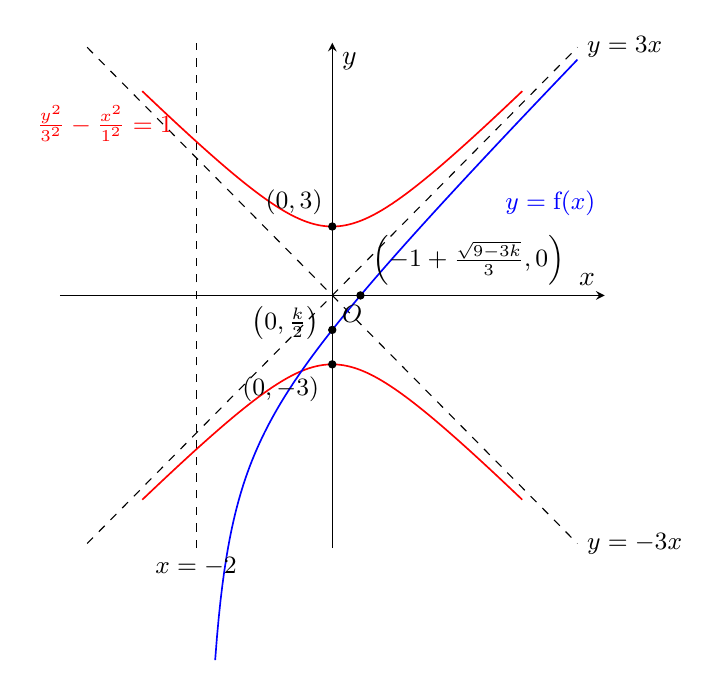
\begin{tikzpicture}
\begin{axis}[width=8.5cm,height=8cm,axis lines=middle,xmin=-4,xmax=4,ymin=-11,ymax=11,ticks=none,clip=false,xlabel=$x$,ylabel=$y$]
\addplot[black,dashed] coordinates{(-2,-11)(-2,11)};
\addplot[black,dashed,domain=-3.6:3.6]{3*x};
\addplot[black,dashed,domain=-3.6:3.6]{-3*x};
\addplot[red,semithick,domain=-1.75:1.75,samples=100,variable=\t]({sinh(t)},{3*cosh(t)});
\addplot[red,semithick,domain=-1.75:1.75,samples=100,variable=\t]({sinh(t)},{-3*cosh(t)});
\addplot[blue,semithick,domain=-1.72:3.6,samples=200]{3*x-3/(x+2)};
\addplot[black,only marks,mark=*,mark size=1.3pt] coordinates{(0,-1.5)(0.414,0)(0,3)(0,-3)};
\node[font=\small,anchor=north west] at (axis cs:0,0){$O$};
\node[font=\small,anchor=east] at (axis cs:-0.05,-1.2){$\left(0,\frac{k}{2}\right)$};
\node[font=\small,anchor=south west] at (axis cs:0.45,0){$\left(-1+\frac{\sqrt{9-3k}}{3},0\right)$};
\node[font=\small,anchor=south east] at (axis cs:0,3.1){$(0,3)$};
\node[font=\small,anchor=north east] at (axis cs:-0.05,-3.1){$(0,-3)$};
\node[font=\small,anchor=north] at (axis cs:-2,-11){$x=-2$};
\node[font=\small,anchor=west] at (axis cs:3.6,10.8){$y=3x$};
\node[font=\small,anchor=west] at (axis cs:3.6,-10.8){$y=-3x$};
\node[font=\small,anchor=west,blue] at (axis cs:2.4,4){$y=\mathrm{f}(x)$};
\node[font=\small,anchor=east,red] at (axis cs:-2.2,7.5){$\frac{y^{2}}{3^{2}}-\frac{x^{2}}{1^{2}}=1$};
\end{axis}\end{tikzpicture}\end{center}
\begin{topalign}
y=\mathrm{f}(x)\ \text{and}\ \frac{y^{2}}{3^{2}}-\frac{x^{2}}{1^{2}}=1\ &\text{have one intersection point}\\
\therefore\ (*)\ \text{has one real root}&
\end{topalign}
\end{qparts}}
%% ============================================================ 34  RVHS 2025 Prelim P1 Q12
\defQ{34}{}{%
The curve $C$ is defined by the parametric equations $x=6t-5$ and $y=2t^{2}+1$, where $t\geqslant\dfrac56$.
\begin{qparts}
\pt{(a)} Sketch the curve $C$, labelling the exact coordinates of any axial intercept(s). \mk{1}
\pt{(b)} Find the equation of the normal to $C$ at the point $P$ where $t=1$. \mk{2}
\pt{(c)} Find the acute angle between the normal to $C$ at the point $P$ where $t=1$ and the tangent to $C$ at the point $M$ where $t=3$. \mk{2}
\pt{(d)} The curve $C$ is translated 5 units in the positive $x$-direction and translated 3 units in the negative $y$-direction, to form the curve $D$. Find the equation of $D$ in parametric form. \mk{2}
\end{qparts}
The curve $E$ is defined by the parametric equations $x=7u$ and $y=\dfrac{9}{u}$, where $u\neq0$.
\begin{qparts}
\pt{(e)} Show that at the point of intersection of the curves $C$ and $E$, $6t^{3}-5t^{2}+3t-34=0$.
Deduce that there is only one point of intersection and find the coordinates of this point. \mk{4}
\end{qparts}
\src{RVHS 2025 Prelim P1 Q12}}
\defS{34}{%
\begin{qparts}
\pt{(a)} \begin{topalign}
t=\frac56:\quad x=6\left(\frac56\right)-5=0,\quad y=2\left(\frac56\right)^{2}+1&=\frac{43}{18}\\
\text{Endpoint (}y\text{-intercept): }&\left(0,\frac{43}{18}\right)
\end{topalign}
\begin{center}\begin{tikzpicture}
\begin{axis}[width=7cm,height=6cm,axis lines=middle,xmin=-10,xmax=22,ymin=-6,ymax=30,ticks=none,clip=false,xlabel=$x$,ylabel=$y$]
\addplot[red,semithick,domain=0.8333:3.6,samples=100,variable=\t]({6*t-5},{2*t^2+1});
\addplot[red,only marks,mark=*,mark size=1.4pt] coordinates{(0,2.389)};
\addplot[black,only marks,mark=*,mark size=1.3pt] coordinates{(7,9)};
\node[font=\small,anchor=north east] at (axis cs:0,0){$O$};
\node[font=\small,anchor=east] at (axis cs:-0.3,2.6){$\left(0,\frac{43}{18}\right)$};
\node[font=\small,anchor=west] at (axis cs:7.4,10){$(7,9)$};
\node[font=\small,red,anchor=west] at (axis cs:16.6,26){$C$};
\end{axis}\end{tikzpicture}\end{center}
\pt{(b)} \begin{topalign}
\frac{\mathrm{d}x}{\mathrm{d}t}=6,\quad \frac{\mathrm{d}y}{\mathrm{d}t}&=4t\\
\frac{\mathrm{d}y}{\mathrm{d}x}&=\frac{4t}{6}=\frac23t\\
t=1:\quad \frac{\mathrm{d}y}{\mathrm{d}x}=\frac23\ &\Rightarrow\ \text{gradient of normal}=-\frac32\\
t=1:\quad x=1,\ y&=3\\
y-3&=-\frac32(x-1)\\
y&=-\frac32x+\frac92
\end{topalign}
\pt{(c)} \begin{topalign}
t=3:\quad \text{gradient of tangent}&=\frac23(3)=2\\
\theta_{1}+\theta_{2}&=\tan^{-1}(2)-\tan^{-1}\left(-\frac32\right)=2.089942\ \text{or}\ 119.7^{\circ}\\
\text{Acute angle}&=\pi-2.089942\ \text{or}\ 180^{\circ}-119.7^{\circ}\\
&=1.05\ \text{or}\ 60.3^{\circ}
\end{topalign}
\pt{(d)} \begin{topalign}
x-5=6t-5\ &\Rightarrow\ x=6t\\
y+3=2t^{2}+1\ &\Rightarrow\ y=2t^{2}-2\\
D:\quad x=6t,\ y&=2t^{2}-2
\end{topalign}
\pt{(e)} \begin{topalign}
6t-5=7u\ \Rightarrow\ u&=\frac{6t-5}{7} &&---(1)\\
2t^{2}+1&=\frac{9}{u} &&---(2)\\
\text{Sub (1) into (2): }2t^{2}+1&=\frac{63}{6t-5}\\
\left(2t^{2}+1\right)(6t-5)&=63\\
12t^{3}-10t^{2}+6t-68&=0\\
6t^{3}-5t^{2}+3t-34&=0\quad\text{(shown)}\\
(t-2)\left(6t^{2}+7t+17\right)&=0\\
6t^{2}+7t+17:\ b^{2}-4ac=7^{2}-4(6)(17)&=-359<0\ \Rightarrow\ \text{no real roots}\\
\therefore\ t=2\ \text{only}\ \Rightarrow\ &\text{only one point of intersection}\\
t=2:\quad x=6(2)-5=7,\ y=2(2)^{2}+1&=9\\
\text{Point of intersection: }&(7,9)
\end{topalign}
\end{qparts}}
%% ============================================================ 35  HCI 2024 Promo Q12
\defQ{35}{}{%
The parametric equations of the curve $C$ are
\[x=\tan\theta-1\quad\text{and}\quad y=2\sec\theta,\quad\text{where }-\frac{\pi}{2}<\theta<\frac{\pi}{2}.\]
\begin{qparts}
\pt{(a)} Find $\dfrac{\mathrm{d}y}{\mathrm{d}x}$ in terms of $\theta$, leaving your answer in a single trigonometric function. \mk{2}
\pt{(b)} Find the equation of the tangent to $C$ at the point where it cuts the $y$-axis, leaving your answer in exact form. \mk{3}
\pt{(c)} Find the Cartesian equation of $C$. \mk{1}
\pt{(d)} Find the equations of the asymptotes and state the coordinates of any turning point(s). \mk{3}
\pt{(e)} The region bounded by the tangent found in part (b), the curve $C$ and the line $x=-1$ is rotated completely about the $x$-axis. Calculate the volume obtained. \mk{3}
\end{qparts}
\src{HCI 2024 Promo Q12}}
\defS{35}{%
\begin{qparts}
\pt{(a)} \begin{topalign}
\frac{\mathrm{d}y}{\mathrm{d}x}&=\frac{\mathrm{d}y}{\mathrm{d}\theta}\div\frac{\mathrm{d}x}{\mathrm{d}\theta}=\frac{2\sec\theta\tan\theta}{\sec^{2}\theta}=2\sin\theta
\end{topalign}
\pt{(b)} \begin{topalign}
x=0:\quad \tan\theta-1=0\ \Rightarrow\ \tan\theta&=1\\
\theta&=\frac{\pi}{4}\quad\text{since}\ -\frac{\pi}{2}<\theta<\frac{\pi}{2}\\
\theta=\frac{\pi}{4}:\quad y=\frac{2}{\cos\frac{\pi}{4}}=2\sqrt2,\quad \frac{\mathrm{d}y}{\mathrm{d}x}=2\sin\frac{\pi}{4}&=\sqrt2\\
\text{Tangent: }y&=\sqrt2x+2\sqrt2
\end{topalign}
\pt{(c)} \begin{topalign}
\tan^{2}\theta+1&=\sec^{2}\theta\\
(x+1)^{2}+1&=\left(\frac{y}{2}\right)^{2}\\
-\frac{\pi}{2}<\theta<\frac{\pi}{2}\ \Rightarrow\ 0<\cos\theta\leqslant1\ \Rightarrow\ \sec\theta\geqslant1\\
\therefore\ (x+1)^{2}+1=\left(\frac{y}{2}\right)^{2},\quad y&\geqslant2
\end{topalign}
\pt{(d)} \begin{topalign}
\text{Asymptotes: }\left(\frac{y}{2}\right)^{2}&=(x+1)^{2}\\
\frac{y}{2}&=\pm(x+1)\\
y=2x+2\quad\text{or}\quad y&=-2x-2\\
\text{Centre }(-1,0),\ y\geqslant2\ \Rightarrow\ &\text{turning point }(-1,2)
\end{topalign}
\begin{center}\begin{tikzpicture}
\begin{axis}[width=7cm,height=6.5cm,axis lines=middle,xmin=-4.5,xmax=2.5,ymin=-3,ymax=8,ticks=none,clip=false,xlabel=$x$,ylabel=$y$]
\addplot[black,dashed,domain=-4.5:2.5]{2*x+2};
\addplot[black,dashed,domain=-4.5:2.5]{-2*x-2};
\addplot[black,dashed] coordinates{(-1,-3)(-1,8)};
\addplot[red,semithick,domain=-1.1:2.2,samples=100]{sqrt(2)*x+2*sqrt(2)};
\addplot[blue,semithick,domain=-1.33:1.33,samples=150,variable=\t]({tan(deg(t))-1},{2/cos(deg(t))});
\fill[orange!60,opacity=0.6] (axis cs:-1,2)--plot[domain=-1:0,samples=30] (axis cs:\x,{2*sqrt((\x+1)^2+1)})--(axis cs:0,2.828)--(axis cs:-1,1.414)--cycle;
\addplot[black,only marks,mark=*,mark size=1.3pt] coordinates{(-1,2)(0,2.828)};
\node[font=\small,anchor=north east] at (axis cs:0,0){$O$};
\node[font=\small,anchor=east] at (axis cs:-1.2,2.3){$(-1,2)$};
\node[font=\small,anchor=west] at (axis cs:0.1,2.5){$\left(0,2\sqrt2\right)$};
\node[font=\small,anchor=south] at (axis cs:-1,8){$x=-1$};
\node[font=\small,anchor=west] at (axis cs:2.5,7){$y=2x+2$};
\node[font=\small,anchor=east] at (axis cs:-4.5,7){$y=-2x-2$};
\node[font=\small,anchor=west,red] at (axis cs:2.2,5.9){$y=\sqrt2x+2\sqrt2$};
\end{axis}\end{tikzpicture}\end{center}
\pt{(e)} \begin{topalign}
\frac{y^{2}}{4}&=(x+1)^{2}+1\\
y^{2}&=4(x+1)^{2}+4\\
\text{Volume}&=\pi\int_{-1}^{0}\left[4\left((x+1)^{2}+1\right)-\left(\sqrt2x+2\sqrt2\right)^{2}\right]\mathrm{d}x\\
&=2.09\ \text{units}^{3}
\end{topalign}
\end{qparts}}
